\section{Program \texttt{lalapps\_animate}}
\label{program:lalapps-animate}
\idx[Program]{lalapps\_animate}

\begin{entry}

\item[Name]
\verb$lal_animate$ --- produces an animated display showing the time
series output of a selected channel in a lower window, and a simultaneously
calculated FFT power spectrum in the upper window

\item[Synopsis]
\verb$lal_animate$ [\verb$--help$] [\verb$--channel$ \textit{name}] 
[\verb$--duration$ \textit{secs}] [\verb$--epoch$ \textit{sec}
\textit{nsec}] [\verb$--framedir$ \textit{dirname}] 
[\verb$--highpass$ \textit{freq} \textit{attenuation}]
[\verb$--numpts$ \textit{npoints}] $|$ xmgr -pipe

%              "    --help                Print this help message\n" \
%              "    --channel name        Name of frame channel\n" \
%              "   [--duration secs]      How many seconds to look at\n"\
%              "   [--epoch sec nsec]     The starting epoch\n"\
%              "   [--framedir dirname]   Directory containing frame files\n"\
%              "   [--highpass freq attenuation]  High-pass filter parameters \n"\
%              "   [--numpts npoints]     Points per graph displayed\n"

\item[Description]
\verb$lal_animate$ produces an animated display showing the time
series output of a selected channel in a lower window, and a simultaneously
calculated FFT power spectrum in the upper window.  The output from
this program must be piped into the graphing program \texttt{xmgr}.

\item[Options]\leavevmode
\begin{entry}
\item[\texttt{--help}]
Print a help message.
\item[\texttt{--channel} \textit{name}]
Name of frame channel
\item[\texttt{--duration} \textit{secs}] 
How many seconds to look at
\item[\texttt{--epoch} \textit{sec} \textit{nsec}] 
Starting epoch
\item[\texttt{--framedir} \textit{dirname}] 
Directory containing frame files
\item[\texttt{--highpass} \textit{freq} \textit{attenuation}]
High-pass filter parameters
\item[\texttt{--numpts} \textit{npoints}]
Points per graph to display
\end{entry}

\item[Example]
To run the program,  type:
\begin{verbatim}
lalapps_animate --channel H2:LSC-AS_Q --framedir ./h1 --numpts 16384 \
--epoch 693768272 0 --duration 1 --highpass 300 0.01 | xmgr -pipe
\end{verbatim}
This will search in directory \verb$./h1$ for frame files containing
the channel \verb$H2:LSC-AS_Q$ and pipe the data starting at 693768272
GPS seconds and 0 GPS nanonseconds to xmgr in segments containing 16384 
points until 1 seconds of data has been reviewed.  The data is highpass 
filtered to above 300 Hz with an attenuation of $0.1$;  the output is
shown in Fig.~\ref{f:animate}
\begin{figure}[h]
\label{f:animate}
\caption{Example of output from \texttt{lalapps\_animate} program}
\begin{center}
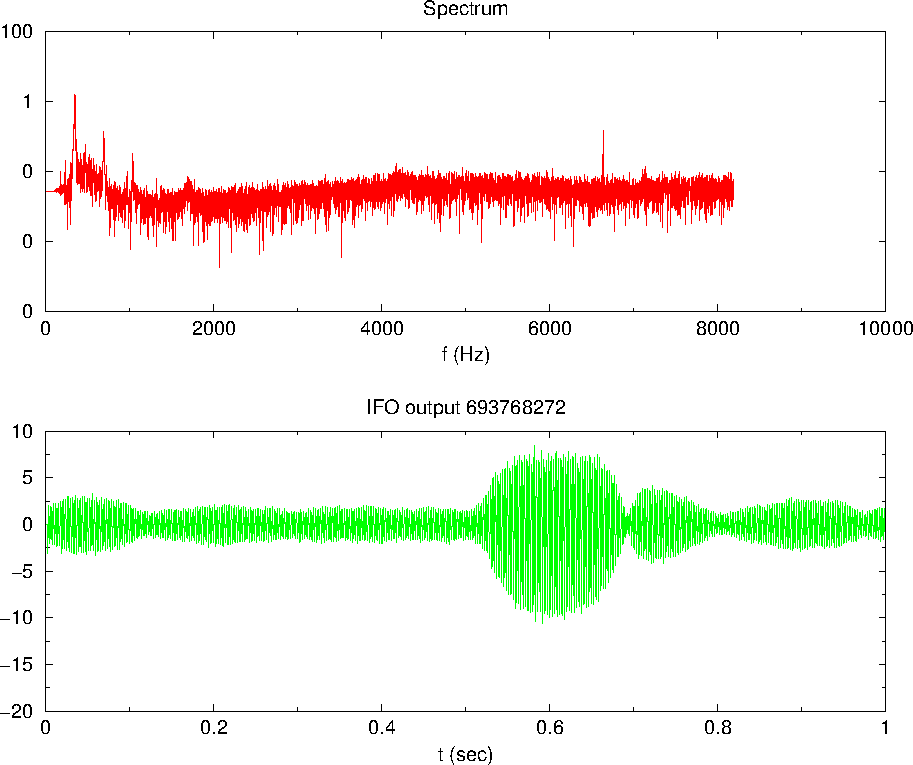
\includegraphics[angle=-90,width=400pt]{animate}
\end{center}
\end{figure}

\item[Author]
Bruce Allen and Patrick Brady

\end{entry}
